\claude{
\section{Applied experiments: monitoring learned simplification}\label{sec:applied}
We evaluate three practical uses: detecting restrictions on parameter updates, tracking information loss in a representation, and measuring changes in learned behavior. Each experiment defines simplification through an independent reference. The test is whether MG detects that change from a scalar record, even when its absolute value has no established dimension interpretation.

\subsection{CNN training: detecting restrictions on parameter updates}\label{sec:cnn}
We train a 14,666-parameter convolutional neural network (CNN) on 10,000 CIFAR-10 images \citep{krizhevsky2009learning} for 10,000 SGD updates. At update 4,000, we reduce the learning rate, freeze layers, or prune weights. Controls continue unchanged, increase the batch size, or transform the observed log by rescaling or smoothing without altering training. MG receives only the norm of all parameters, which requires no extra network forward pass. Settings are $W=1,000$, stride 500, $E=20$, $\tau=1$, and $k=20$.

We calibrate on seeds 0--3 and test interventions of different strengths on new seeds 10--13. Independent measurements record the covariance participation ratio of updates, the fraction of parameters that move, and update magnitude. Freezing and pruning impose known restrictions on trainable or nonzero parameters. Learning-rate reduction changes the dynamics, but need not reduce invariant dimension; we assess its effect through the measured updates.

MG falls after strong restrictions on training. Freezing all but the classification head reduces it by a median 18.5\%, while update participation ratio falls by 43.5\%. Strong freezing and pruning produce median MG declines of approximately 12--19\%; control medians range from near zero to increases of 13\%. Across intervention strengths, MG ratios and update participation-ratio changes have Spearman correlation 0.59. They measure different aspects of the change: after 50\% pruning, MG falls while update participation ratio rises.

\begin{figure*}[t]
\centering
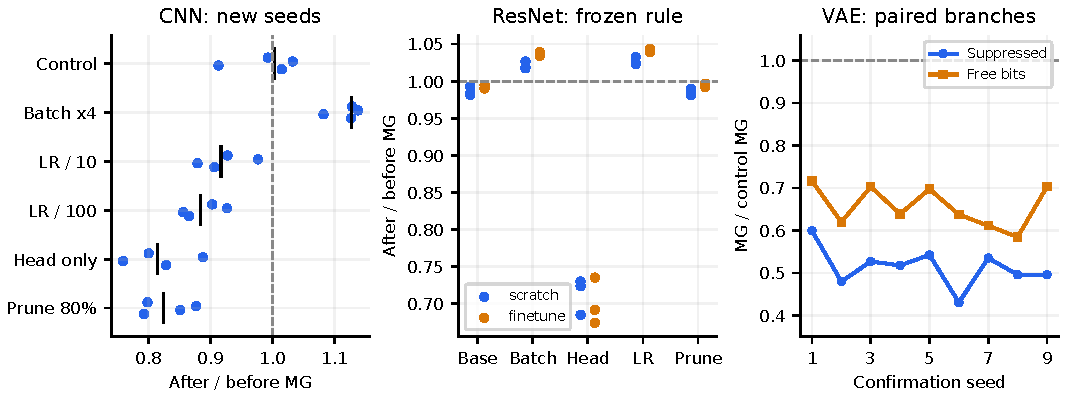
\includegraphics[width=.98\textwidth]{figures/applications.pdf}
\caption{\claude{MG tracks changes across learning tasks. Left: CNN estimates after an intervention divided by those before it, on four held-out seeds. Bars show medians; the dashed line means no change. Center: the same comparison for ResNet-18 trained from scratch or pretrained weights, with all seeds shown. Right: late MG in the suppressed and free-bits VAE branches relative to their shared low-regularization control, across nine test seeds. Independent update and information measurements validate the changes.}}
\label{fig:applications}
\end{figure*}

\paragraph{MG adds information beyond simple scalar statistics.}
MG separates the graded interventions from unchanged-training and increased-batch controls with area under the ROC curve (AUC) 0.93. Trend crossings, lag-one autocorrelation, and detrended standard deviation achieve 0.48--0.57 on the same comparison. Comparing only the strongest intervention doses against all specified controls gives MG an AUC of 0.99.

As a further check, we apply MG to surrogate records generated by iterative amplitude-adjusted Fourier transforms (IAAFT). These preserve the marginal distribution and approximately the spectrum, but yield AUC 0.68. The stronger separation in the original records suggests that these properties alone do not explain the result. All comparisons use the same records and a direction of change fixed before evaluation.

\paragraph{Detecting changes using only past observations.}
For window estimates $m_j$, we compare the median over the latest $M$ windows with the median over the preceding $B$ windows:
\begin{equation}
D_j=\frac{\median(m_{j-M+1},\ldots,m_j)}
{\median(m_{j-M-B+1},\ldots,m_{j-M})}-1.
\label{eq:detector}
\end{equation}
Calibration selects $M=2$, $B=3$, and an alarm threshold of $D_j<-0.0883$, a drop of 8.83\%. Only completed windows enter the rule. We count the first threshold crossing as an alarm and score it as a detection if it occurs within 5,000 updates after the intervention. An earlier alarm is false. Competing statistics use the same calibration procedure.

MG detects 27/28 strong interventions with no alarms in 16 control records and median delay 1,000 updates (Table~\ref{tab:detectors}). Standard deviation detects all 28 but raises alarms in 10/16 controls; trend crossings detect 15/28 with 5/16 control alarms. MG therefore combines high detection with fewer false alarms on this benchmark. Weak interventions are less reliably detected. The records share four seeds, so these counts are not independent trials. We evaluate detection here; whether acting on an alarm improves training requires a separate test.

\begin{table}[t]
\centering\small
\caption{\claude{MG detects most strong CNN interventions with no control alarms. All methods are calibrated on the same earlier seeds and evaluated on four new seeds. ``Alarms'' counts control records with an alarm. Delay is measured only for detected events.}}
\label{tab:detectors}
\begin{tabular}{lrrr}
\toprule
Statistic & Detected & Alarms & Delay \\
\midrule
MG & 27/28 & 0/16 & 1,000 \\
Trend crossings & 15/28 & 5/16 & 1,000 \\
Lag-one correlation & 0/28 & 0/16 & --- \\
Detrended std. & 28/28 & 10/16 & 500 \\
\bottomrule
\end{tabular}

\end{table}

\subsection{Transferring the detector to ResNet-18}
We transfer the parameter-norm observable, MG settings, and alarm threshold to ResNet-18 \citep{he2016deep}, without recalibration. Training uses the full CIFAR-10 training set, either from scratch or from ImageNet-pretrained weights, with three new seeds in each setting. Freezing the backbone while continuing to train the head reduces MG by a median 27.6\% and 30.8\%, respectively. The detector identifies all six freezing events with no alarms in 24 control records.

This transfers a detector from about 15 thousand to 11 million parameters for a concrete training change. The global parameter norm is informative for backbone freezing, but the same detector misses the tested learning-rate reductions and pruning interventions in ResNet-18. Separately explored layer norms and random projections introduce false alarms. Thus transfer succeeds for the freezing task, while other interventions require further validation of the observable and detector.

\subsection{Text VAE: tracking information loss and preservation}\label{sec:vae}
A text variational autoencoder (VAE) learns to reconstruct Penn Treebank sentences \citep{marcus1993building} through a 16-dimensional Gaussian latent code. Its encoder and decoder use gated recurrent units \citep{bowman2016generating}; the model has 276,016 parameters and trains on 6,000 sentences. This task tests whether MG can reveal when the decoder stops using information in the code.

After 1,024 shared updates with Kullback--Leibler (KL) regularization weight $\beta=0.01$, we split training into three branches: keep that weight, raise it to one, or use $\beta=1$ with a free-bits objective. Free bits reduces pressure to suppress low-KL latent coordinates. All branches train until update 3,072.

MG uses the reconstruction negative log-likelihood (NLL) per token on 16 fixed validation sentences, with fixed latent sampling noise. It has no access to KL or the independent references. On a larger set of 256 validation sentences, the references estimate latent mutual information and the decoder's response to shuffling codes between sentences. A joint decline means that less information is retained and used through the latent code.

The information-loss criterion is met on all nine test seeds. MG declines more strongly in the high-regularization branch than in its control on every seed: their median late MG ratio is 0.517, with a 95\% seed-bootstrap interval [0.480, 0.542]. Free bits partially preserves both information and decoder dependence. MG is then higher than in the suppressed branch on all nine seeds, with median ratio 1.286 [1.179, 1.418]. The preservation control is informative because the two branches use the same external KL weight but retain different amounts of information. MG distinguishes these outcomes from reconstruction logs alone.

This result validates MG as a signal of latent information loss and partial preservation. Standard deviation and spectral entropy also detect the loss on all nine seeds. In a separate cyclic-VAE test, using MG to schedule expensive reference checks finds 28/41 transitions at the primary budget, compared with 38/41 for periodic checks. Association with information loss therefore does not by itself imply better scheduling. The CNN benchmark provides the clearest detection advantage over simple scalar statistics.

\subsection{Grokking and learned control}
\paragraph{Grokking.}
In modular-arithmetic training, scalar parameter-norm MG falls near generalization in all four positive runs when its temporal resolution is matched to that of the trajectory analysis. Independently, saved trajectory sketches show a sharp, reversible collapse of detrended covariance participation ratio. Across settings applied to these same runs, 24/26 usable comparisons distinguish the positive runs from two controls. These comparisons are not independent repetitions. Roughness changes are stronger, a memorizing control also simplifies, and the full-batch setting does not reproduce the same scalar result. The evidence supports sensitivity to a training transition, without making an MG decline a unique indicator of generalization.

\paragraph{Learned locomotion.}
We also analyze behavior learned by proximal policy optimization (PPO) in Walker2d \citep{schulman2017proximal,todorov2012mujoco}. At fixed policy checkpoints, we compute MG from a scalar joint or control signal. Two series of five fine-tuning seeds show lower control-log MG under moderate action smoothing. In the final comparison, median ratios to the control are 0.801 and 0.604 for two penalty strengths, with a decline on every seed. This extends the scalar analysis from training logs to learned behavior. Full-state repeatability and perturbation tests show that simpler control signals do not consistently imply a simpler full-body gait. Simple increment and return statistics remain competitive; Appendix~\ref{app:additional} gives the comparisons and shared-initial-policy design.
}
